\documentclass[11pt]{article}

\input{preambulo.tex}

\usepackage{booktabs}
\usepackage{multirow}
\usepackage{listings}
\usepackage{xcolor}
\usepackage{subcaption}
\usepackage[table]{xcolor}
\usepackage{titlesec}

\colorlet{maincolor}{Violet}

% Definición de colores pastel y modernos
\definecolor{backcolour}{rgb}{0.96,0.96,0.96}
\definecolor{codegreen}{rgb}{0.13,0.55,0.13}
\definecolor{codegray}{rgb}{0.5,0.5,0.5}
\definecolor{codepurple}{rgb}{0.58,0,0.82}
\definecolor{codeblue}{rgb}{0.0,0.0,0.8}

% Configuración del estilo moderno
\lstdefinestyle{modern}{
    backgroundcolor=\color{backcolour},   
    commentstyle=\color{codegreen}\itshape,
    keywordstyle=\color{codeblue}\bfseries,
    numberstyle=\tiny\color{codegray},
    stringstyle=\color{codepurple},
    basicstyle=\ttfamily\scriptsize,
    breakatwhitespace=false,         
    breaklines=true,                 
    captionpos=b,                    
    keepspaces=true,                 
    numbers=left,                    
    numbersep=10pt,                  
    showspaces=false,                
    showstringspaces=false,
    showtabs=false,                  
    tabsize=4,
    frame=single,                    % Marco simple alrededor del código
    rulecolor=\color{lightgray},     % Color del marco
    xleftmargin=15pt,                % Margen para que los números no se peguen
    literate={á}{{\'a}}1 {é}{{\'e}}1 {í}{{\'i}}1 {ó}{{\'o}}1 {ú}{{\'u}}1
             {Á}{{\'A}}1 {É}{{\'E}}1 {Í}{{\'I}}1 {Ó}{{\'O}}1 {Ú}{{\'U}}1
             {ñ}{{\~n}}1 {Ñ}{{\~N}}1
}

% Aplicar el estilo por defecto a todos los bloques de código
\lstset{style=modern}

% --- CONFIGURACIÓN DE SECCIONES ---

% Formato para \section
% Sintaxis: \titleformat{\comando}{formato}{etiqueta}{separación}{antes_del_texto}
\titleformat{\section}
  {\color{maincolor}\large\bfseries} % Color, fuente, tamaño y estilo
  {\thesection.} % Muestra el número de sección (ej. 1, 2...)
  {0.5em} % Espacio entre el número y el texto del título
  {} % Código adicional antes del texto del título

% Formato para \subsection
\titleformat{\subsection}
  {\color{maincolor}\large\bfseries} % Color vino, tamaño grande, cursiva
  {\thesubsection}
  {0.5em}
  {}

\title{}
\author{Jesús Muñoz Velasco}
\date{Curso 2025-2026}

\begin{document}

{\Large \bfseries \centering \color{maincolor} Práctica 1: Uso de IA generativa}

\vspace{0.25cm}
{\large \bfseries \color{maincolor} Autor: Jesús Muñoz Velasco}

Sin duda el principal uso que se ha dado a la IA generativa\footnote{En mi caso he usado Gemini con el modelo Pro.} ha sido la corrección de errores en el código (en especial fallos lógicos). También la he usado para consultar cuáles serían las mejores estructuras de datos para ciertas variables de los algoritmos (abiertos, cerrados, etc). Quiero destacar las siguientes interacciones con la IA que quitando la corrección de fallos han sido las más interesantes:

\begin{flushright}
    
\includegraphics[width=9cm]{img/consultaIA1.png}
\end{flushright}
\begin{flushleft}
    
\includegraphics[width=15cm]{img/consultaIA1_res1.png}
    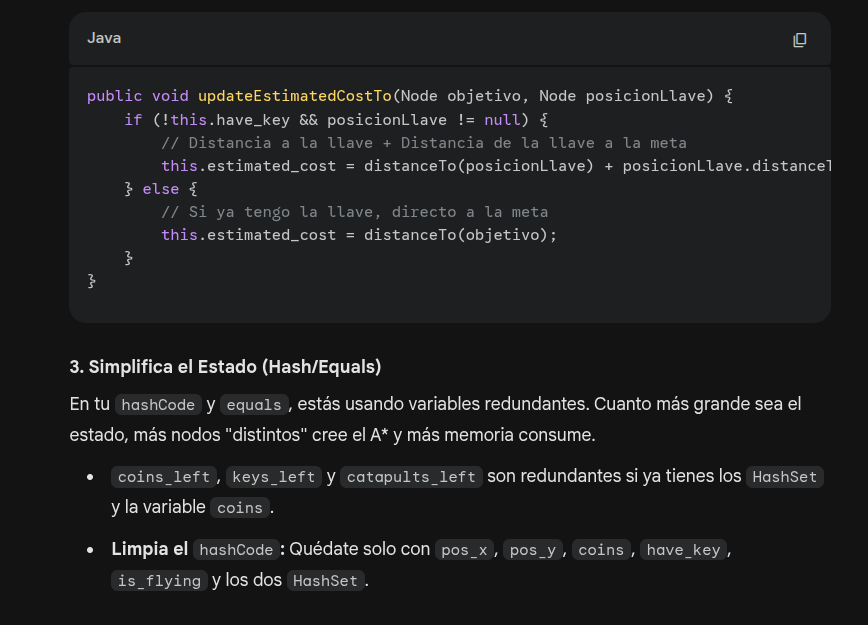
\includegraphics[width=15cm]{img/consultaIA1_res2.png}
    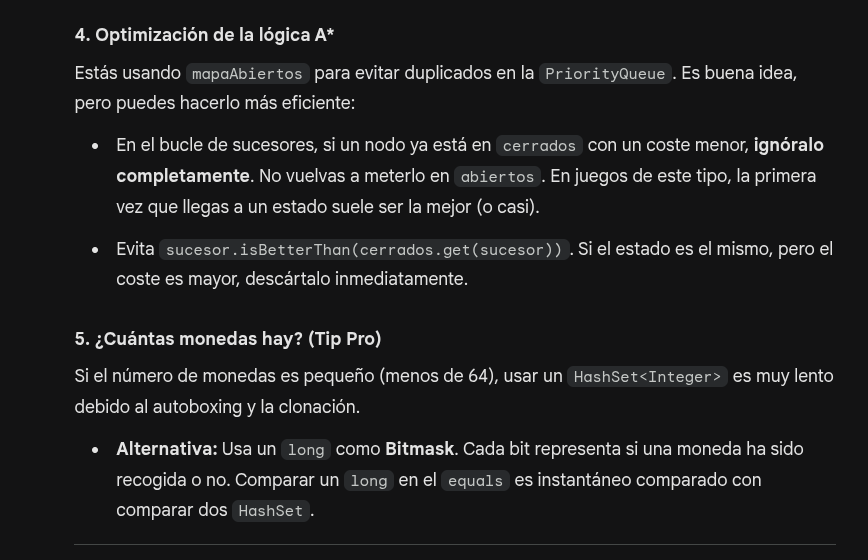
\includegraphics[width=15cm]{img/consultaIA1_res3.png}
\end{flushleft}
Sin duda lo más destacable de esta respuesta fue el punto 5 (el resto había cosas como la heurística que no podía cambiar por el enunciado de la práctica). Me sugirió usar un \textit{bitmask} (máscara de bits) para optimizar la copia de los nodos (ya que antes tenía un \textit{hashset} para almacenar las monedas y catapultas recogidas, y más tarde para las llaves también). Esto hacía muchísimo más eficiente todo. La siguiente consulta fue cómo implementar esto y cómo funcionaba (la parte de la implementación no la adjunto como imágenes porque es muy larga y es como ha quedado en mi código finalmente):

\begin{flushright}
    
\includegraphics[width=9cm]{img/consultaIA2.png}
\end{flushright}
\begin{flushleft}
    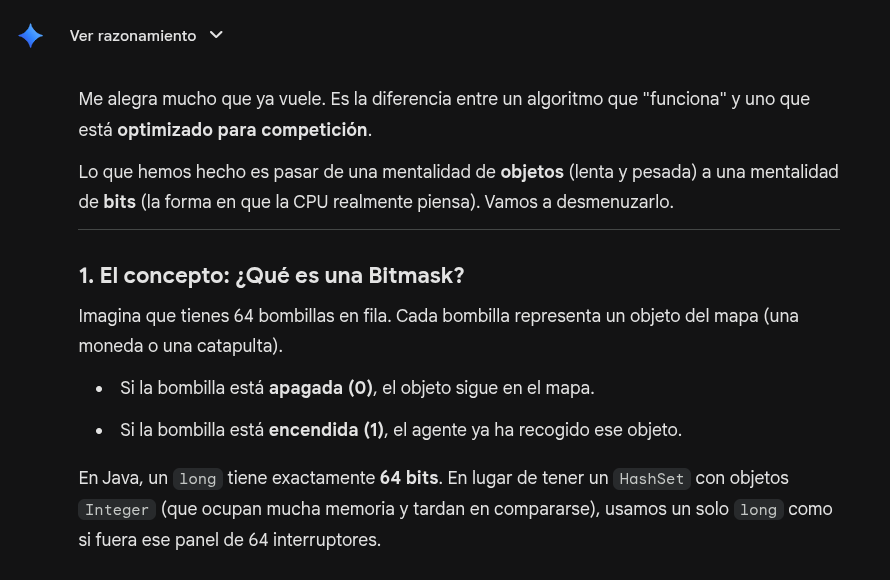
\includegraphics[width=15cm]{img/consultaIA2_res1.png}
    
\includegraphics[width=15cm]{img/consultaIA2_res2.png}
    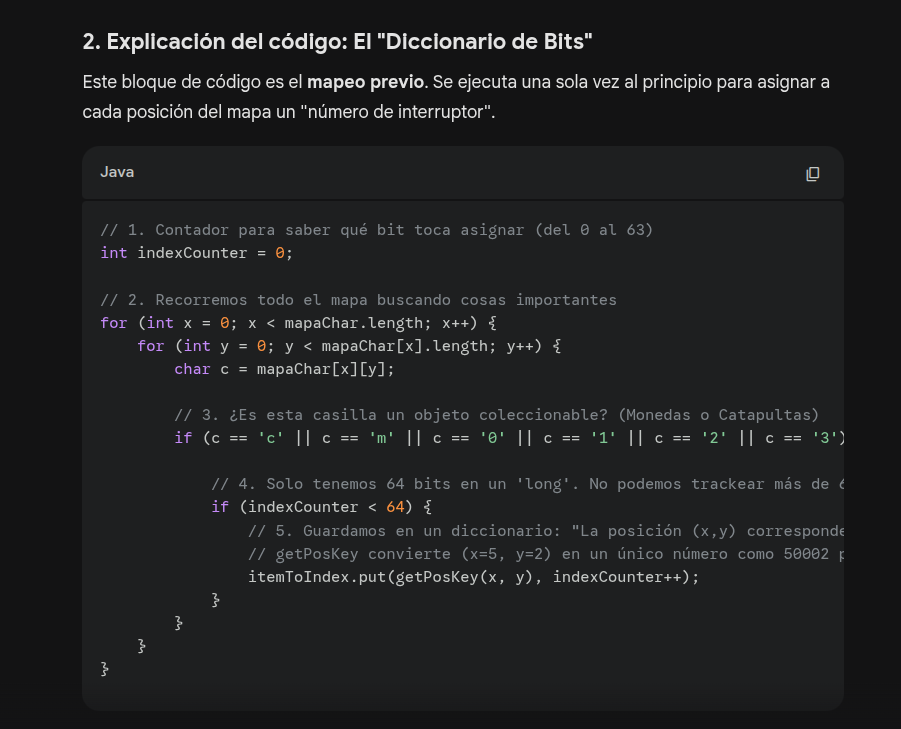
\includegraphics[width=15cm]{img/consultaIA2_res3.png}
    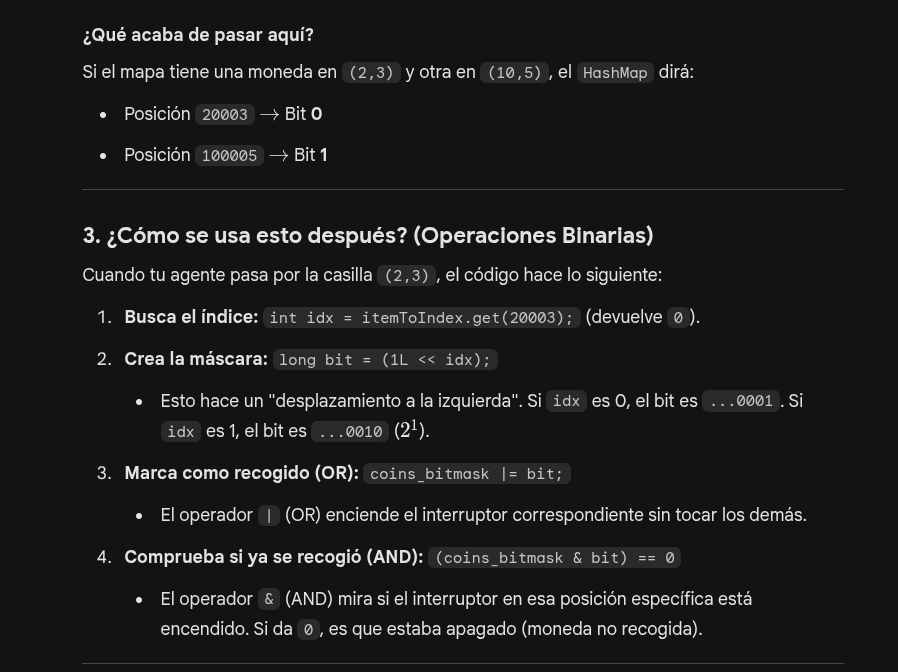
\includegraphics[width=15cm]{img/consultaIA2_res4.png}
    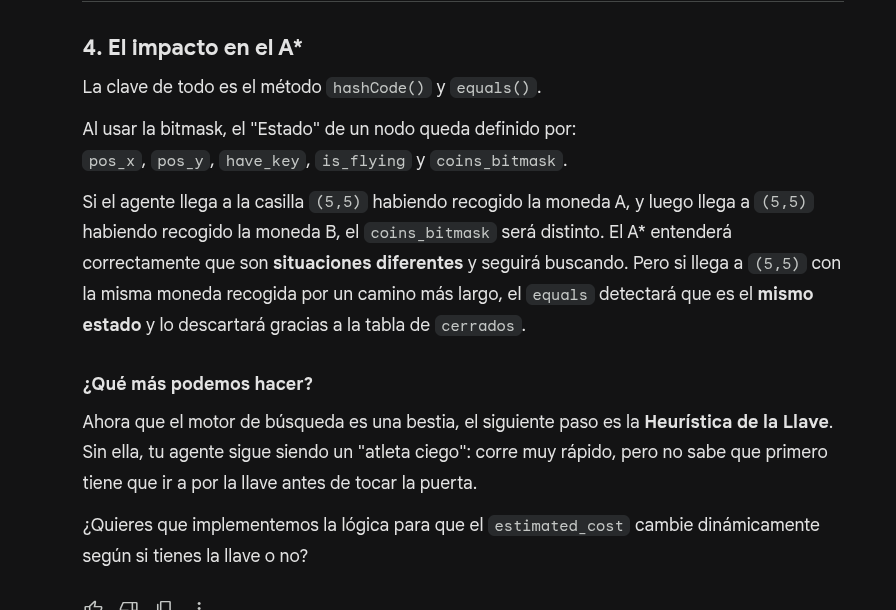
\includegraphics[width=15cm]{img/consultaIA2_res5.png}
\end{flushleft}

Ignorando la sugerencia acerca de la mejora de la heurística me resulto muy útil esta representación de ``marcado'' de posiciones visitadas para marcar cada objeto coleccionable. Más tarde tuve que mejorarla para implementar también las posiciones de las llaves que había recogido (ya que sino no me cuadraban las métricas con las de las soluciones administradas). Es la primera vez que uso una máscara de bits en un código propio (lo habíamos usado en FR pero para máscaras de redes) y me ha parecido una forma muy limpia y eficiente de representar esto (consigue que todos los nodos tengan una representación con tipos primitivos, sin estructuras complejas como \textit{hashsets}). \\

Antes de esto también tengo consultas sobre qué estructuras eran las más eficientes para A* (tenía dos \textit{hashmaps} para abiertos y cerrados respectivamente). Podría destacar la siguiente interacción (quizás la pregunta no tenía nada que ver, pero me sirvió la respuesta):
% \begin{flushright}
%     \includegraphics[width=9cm]{img/consultaIA3.png}
% \end{flushright}
\begin{flushleft}
    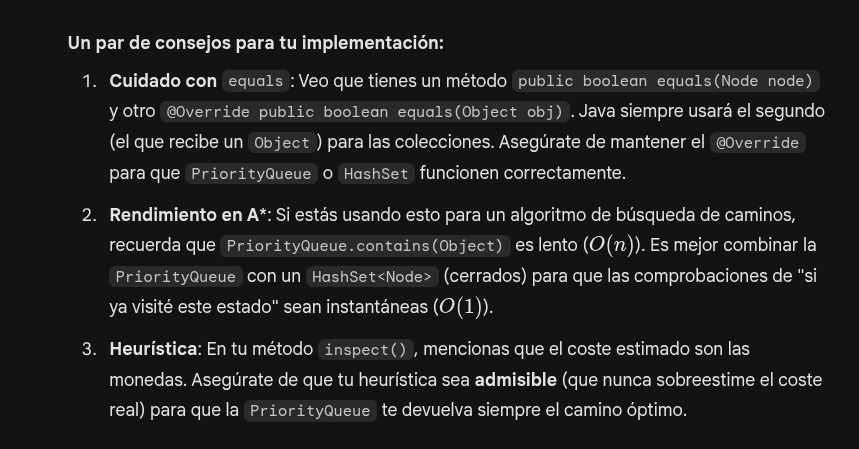
\includegraphics[width=15cm]{img/consultaIA3_res1.png}
%     \includegraphics[width=15cm]{img/consultaIA3_res2.png}
%     \includegraphics[width=15cm]{img/consultaIA3_res3.png}
%     \includegraphics[width=15cm]{img/consultaIA3_res4.png}
\end{flushleft}

Podemos ver que en el punto 2 nos sugiere usar una estructura paralela (resultado que acabé implementando en mi práctica) para la cola con prioridad.\\

Sin duda he usado la IA generativa para muchas más cuestiones, pero han sido sobre todo corrección de errores (ya arreglados en mi código final y sin mayor relevancia). Estas interacciones anteriores son las que más han guiado el desarrollo de mi práctica en cuanto al uso de la IA.

\end{document}
